\chapter{Simulación de tráfico}
\label{ch:sota-traffic-simulation}

El tráfico es un sistema caótico en el que intervienen un número muy elevado de diferentes variables, muchas de las cuales relacionadas entre si. Debido a esto, obtener modelos exactos de tráfico es una tarea prácticamente imposible y es por ello que la mayoría del trabajo cuyo objetivo es la predicción se realice en base a simuladores.

Los simuladores de tráfico son herramientas de software que, usando diferentes modelos, describen el tráfico como sistema, permitiendo:

\begin{itemize}
	\item Extraer resultados y conclusiones de escenarios de tráfico determinados.
	\item Implementar técnicas de tráfico sin necesidad de alterar el tráfico real.
	\item Reproducir exactamente un escenario.
	\item Introducir modificaciones en puntos determinados (e.g. espaciales o temoprales) de un escenario conocido para evaluar la divergencia en su evolución.
\end{itemize}

Los objetivos en la simulación de tráfico son los de hacer que los modelos se parezcan lo máximo posible a la realidad. En este capítulo vamos a ver cuál es la realidad actual de este tipo de simuladores, cuáles son sus diferentes tipologías y maneras de modelar los diferentes aspectos del tráfico y, posteriormente, realizaremos una evaluación de cuáles son los idóneos para nuestro trabajo.

Limitaremos el estudio no obstante a los simuladores de vehículos, obviando otros tipos de simulación de tráfico que no tienen que ver con esta temática, como por ejemplo los orientados a la evaluación de sistemas de señalización inteligentes (e.g.~\cite{jin2016evaluation}) o a la estimación de emisiones (e.g.~\cite{quaassdorff2016microscale}).

\section{Clasificación de simuladores de tráfico}

Los aspectos simulables y medibles del problema tráfico son muy diversos, dependiendo sobre todo del nivel de complejidad del tráfico\sidenote{Modelar una vía por la que circula un centenar de coches no es lo mismo que modelar una ciudad donde circulan millones.}, de qué queremos medir\sidenote{Evaluar a un conductor en una situación determinada o evaluar la evolución del flujo de tráfico en un cuello de botella causado por un accidente.} y de cómo lo modelamos\sidenote{Un autómata celular se modela de forma diferente a un modelo lineal de vías o carriles.}.

El resto de la sección ofrece una visión de las diferentes categorías en las que se clasifican los simuladores de tráfico.

\subsection{Tipos de simulador en función de la complejidad}

La complejidad en una simulación se refiere al nivel de detalle al que queremos llegar a la hora de modelar nuestra solución. Es evidente que según aumentamos el detalle en la simulación aumenta la cantidad de cálculo. Por ejemplo, si queremos modelar el comportamiento de $10$ billones de canicas cayendo por un tubo es considerablemente más eficiente modelarlas como un fluido con una serie de propiedades características que como una colección de elementos individuales, cada uno con sus propiedades (e.g. masa, aceleración, ...) e interaccionando entre sí.

\begin{figure}
	\centering
	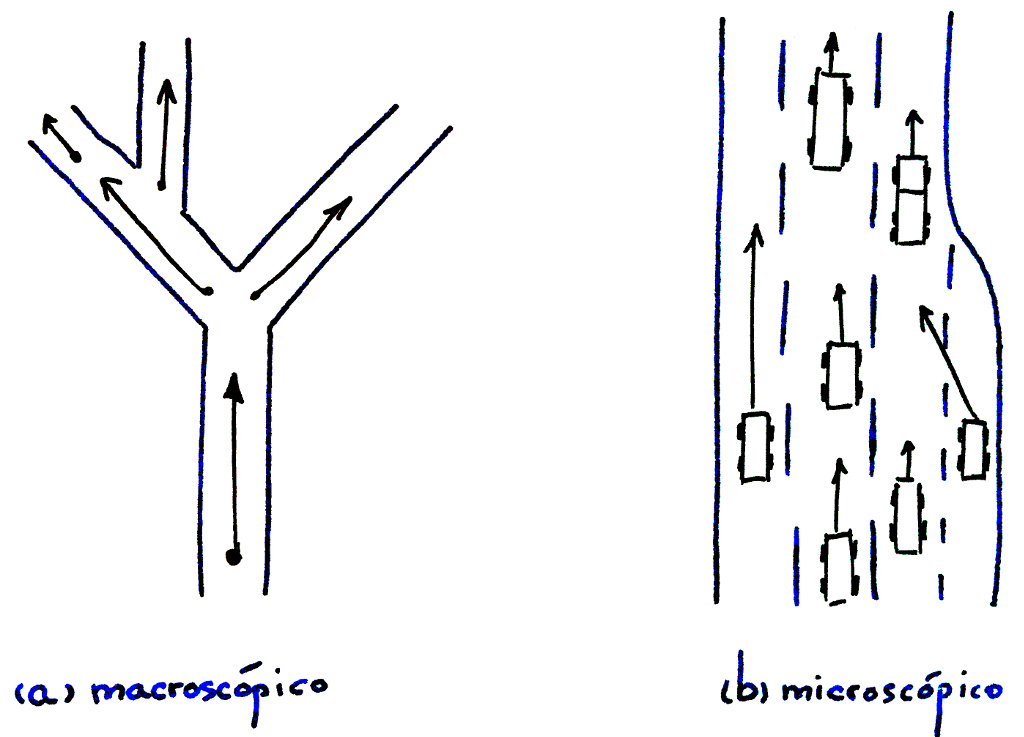
\includegraphics{images/granularities-in-traffic-simulation}
	\caption{Taxonomía clásica de los simuladores en función de la granularidad (complejidad) de la simulación.}
	\label{fig:granularities-in-traffic-simulation}
\end{figure}

En el caso de los simuladores de tráfico es lo mismo. En éstos existe un amplio intervalo de granularidades, desde por ejemplo el flujo de entrada en una autovía hasta el consumo de carburante de un vehículo en ciudad. Lo más común es clasificar los simuladores dentro de dos grandes grupos, los cuales se ilustran en la Figura~\ref{fig:granularities-in-traffic-simulation}:

\begin{itemize}
	\item \textbf{Microsimulación} o simulación de tipo \textbf{micro}. Su objetivo es estudiar, desde un punto de vista de granularidad fina como puede ser vehículos o peatones, las micropropiedades del flujo de tráfico como, por ejemplo, los cambios de carril, las aproximaciones a vehículos delanteros o los adelantamientos, para evaluar su comportamiento. Tiene dos principales ventajas, la posibilidad de estudiar el tráfico como un todo a partir de sus elementos más simples (ofreciendo una representación más fiel de éste) y la posibilidad de estudiar cada elemento por separado. Sin embargo, la principal desventaja de este tipo de modelos es que cada elemento de la simulación requiere de cómputo independiente y por tanto simulaciones con alto contenido de elementos pueden llegar a ser inviables\sidenote{Existen técnicas de computación distribuida que superan ampliamente los límites impuestos por la computación en un único nodo, por ejemplo, el simulador de IBM \textit{Megaffic}. Éste implementa un modelo de granularidad micro donde cada elemento es un agente independiente (i.e. sistema multiagente) usando para ello entornos con cientos de núcleos de proceso que proveen de capacidad suficiente para modelar ciudades enteras como Tokio (ver~\cite{Osogami2012} y~\cite{Suzumura2012}).}.
	\item \textbf{Macrosimulación} o simulación de tipo \textbf{macro}. Este tipo de modelos centran su esfuerzo en estudiar el flujo de tráfico como un todo, explorando sus macropropiedades (e.g. evolución del tráfico, efectos onda, velocidad media o flujo en vías). Su ventaja principal es que a nivel macroscópico permiten estudiar propiedades que a nivel microscópico requeriría una cantidad ingente de recursos. Sin embargo, con este modelo es imposible obtener información precisa de un elemento en particular del tráfico.
\end{itemize}

Aunque esta es la categorización típica de modelos, en la literatura aparecen otros tipos de modelo con granularidades que pueden considerarse no pertenecientes a ninguno de estos dos conjuntos. Este es el caso de los simuladores de tipos \textbf{sub-micro} y los \textbf{meso} (ver figura~\ref{fig:mesoscopic-and-submicroscopic-simulation}). 

\begin{figure}
	\centering
	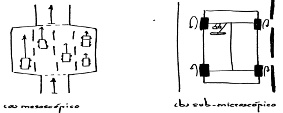
\includegraphics{images/mesoscopic-and-submicroscopic-simulation}
	\caption{Aproximaciones alternativas de modelos en función de la complejidad. Ejemplo de mesosimulación como ventana de microsimulación dentro de un flujo en un macrosimulador (e.g. \cite{munoz2001integrated}) y ejemplo de submicrosimulación donde se modelan componentes internos del vehículo.}
	\label{fig:mesoscopic-and-submicroscopic-simulation}
\end{figure}

Los \textbf{sub-micromodelos} especifican granularidades por debajo del nivel de \enquote{vehículo} o \enquote{peatón}. Por ejemplo, en (\cite{Minderhoud1999}) trabaja a nivel de funcionamiento del control de crucero inteligente de un vehículo en función del entorno del vehículo.

Por otro lado los \textbf{mesosimuladores} (e.g.~\cite{munoz2001integrated} o~\cite{casas2011need}) nacen para amortiguar los problemas inherentes a la complejidad en los micromodelos y a la falta de resolución en los macromodelos.

Dado que en nuestro discurso trabajaremos en la evaluación de modelos de comportamiento de conductores, nos ceñiremos al uso de simuladores que modelen un nivel de granularidad \textbf{micro}.

\subsection{Tipos de simulador en función del espacio y el tiempo}

Existen otras dos formas de clasificar los simuladores en función de cómo evolucionan en la simulación el \textbf{tiempo} y el \textbf{espacio}. Sin embargo, aunque \textit{complejidad}, \textit{tiempo} y \textit{espacio} son dimensiones diferentes a la hora de clasificar simuladores, el tipo de simulador según complejidad determina en gran medida los tipos según las dimensiones espacio y tiempo.

\begin{figure}
	\centering
	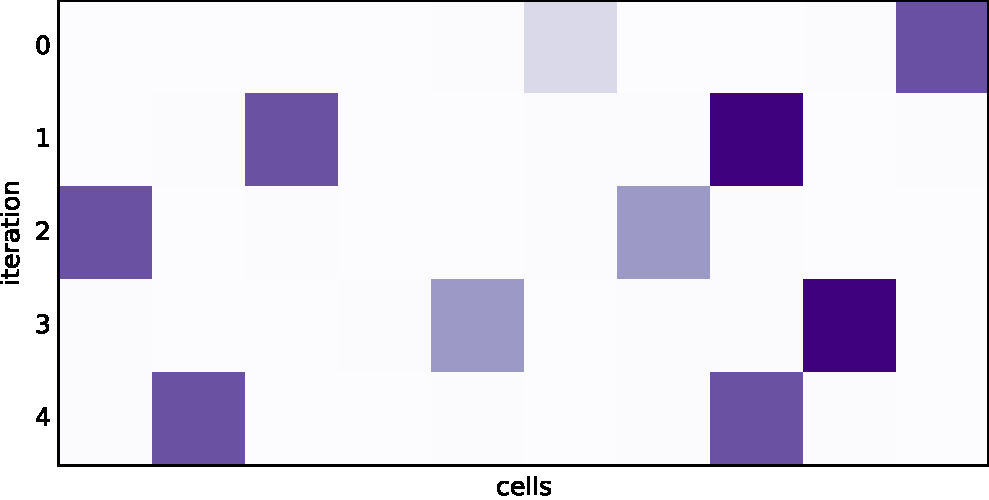
\includegraphics[width=.8\linewidth]{images/cellular-automata-based-sim}
	\caption{Ejemplo de un simulador de tráfico basado en autómatas celulares. En éste, el espacio se divide en celdas que pueden, o bien estar vacías, o bien ocupadas por un vehículo. La ilustración representa la evolución de los tiempos para cada vehículo (representado por un punto) según se desplaza a través del espacio discertizado en celdas de $7.5m$. Concretamente muestra la evolución a lo largo del tiempo del movimiento de un modelo de \textit{car-following} de tres vehículos. Fuente:~\cite{Brilon1999}.}
	\label{fig:cellular-automata-based-sim}
\end{figure}

En el caso del espacio, la clasificación diferencia las simulaciones que se mueven por un espacio discreto o por uno continuo:

\begin{itemize}
	\item De espacio \textbf{discreto}. Simulación donde el espacio está dividido en celdas que nosmalmente sólo pueden estar ocupadas por un elemento en un momento determinado. Este es el caso, por ejemplo, de los simuladores basados en autómatas celulares. La figura~\ref{fig:cellular-automata-based-sim} ilustra el comportamiento de uno de estos tipos de simulador.
	\item De espacio \textbf{continuo}. Simulación que transcurre en una secuencia infinita de puntos en el espacio. Es el caso por ejemplo de los simuladores basados en modelos lineales, como podemos ver en el ejemplo de la figura~\ref{fig:car-following-based-sim}.
\end{itemize}

En el caso del tiempo, la división se realiza en los mismos términos que en los del espacio:

\begin{itemize}
	\item De tiempo \textbf{discreto}. También denominada de \textit{simulación de eventos discretos}, divide el tiempo en intervalos discretos, generalmente (aunque existen excepciones) de longitud fija duranet toda la simulación. Los simuladores basados en autómatas celulares son también simuladores típicos discretos, ya que cada posición en el espacio se va calculando para cada intervalo discreto de tiempo (ver figuras~\ref{fig:cellular-automata-based-sim} y~\ref{fig:nagel-schreck}).
	\item De tiempo \textbf{continuo}. En estos simuladores el tiempo es un factor más para un modelo de ecuaciones diferenciales. La figura~\ref{fig:car-following-based-sim} ilustra un modelo de \textit{car-following} que puede implementarse en una smiulación de tiempo continuo si la aceleración viene determinada por un modelo que entre otros factores incluye el tiempo.
\end{itemize}

\begin{figure}
	\centering
	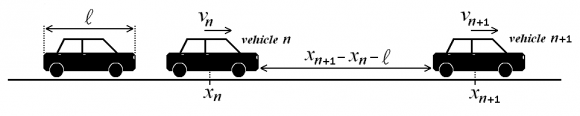
\includegraphics{images/car-following-based-sim}
	\caption{Ejemplo de un modelo lineal en un espacio continuo. La posición del vehículo es un valor $x \in \mathbb{R}$. Este ejemplo representa un modelo de \textit{car-following} donde el comportamiento de la aceleración del vehículo es determinado por la distancia al coche siguiente. Fuente:~\cite{Tordeux2011}.}
	\label{fig:car-following-based-sim}
\end{figure}

En nuestro caso, queremos conocer la situación exacta del vehículo y no una situación aproximada en una separación discreta del espacio. Esto nos dirige hacia simuladores de espacio continuo. Por otro lado, nosotros realizamos la recolección de datos en intervalos cuantificables de tiempo, los cuales serán usados para modelar los comportamientos de los conductores y para contrastar los resultados; por tanto, la elección está sesgada hacia simulación de tiempo discreto.

\section{Modelos de microsimulación}

Si bien es cierto que los sistemas de partículas son usados también para simulación de tráfico microscópico, su ámbito de aplicación es el mismo que el del punto de vista macroscópico, esto es, usar sistemas de partículas para el análisis del tráfico como fluido. Por ello como vertientes principales para representación del tráfico exploraremos los puntos de vista que se ocupan de éste desde el punto de vista del individuo: los autómatas celulares y los sistemas multiagentes.

\subsection{Microsimulación basada en autómatas celulares}

Un autómata celular es una colección ordenada de celdas o \textit{células} $n$-dimensionales que parcelan el universo en estudio. Cada una de dichas celdas se encuentra en un estado (e.g. contiene un valor numérico), y el estado de todas ellas se actualiza síncronamente (esto es, todas a la vez) en intervalos regulares de tiempo denominados \textit{ciclos}. El camio de estado de cada célula depende de los valores de las células vecinas y del algoritmo de modificación al que responden todas y cada una de las células.\sidenote{Hay realmente máquinas capaces de operar de esta manera, es decir, arquitecturas basadas en autómatas celulares. En ellas, cada ciclo de reloj actualiza todas las celdas de memoria del autómata. Éstas arquitecturas se suelen usar para la implementación de modelos físicos \TODO{buscar referencias}, superando en varios órdenes de magnitud la capacidad computacional de las arquitecturas tradicionales.}.

Estos modelos de microsimulación, debido a la propia naturaleza de los autómatas celulares, se encuentran clasificados como simuladores de tiempo y espacio discretos, y se usa debido a su facilidad de implementación y su eficiencia, ya que es fácilmente paralelizable.


\begin{figure}
	\centering
	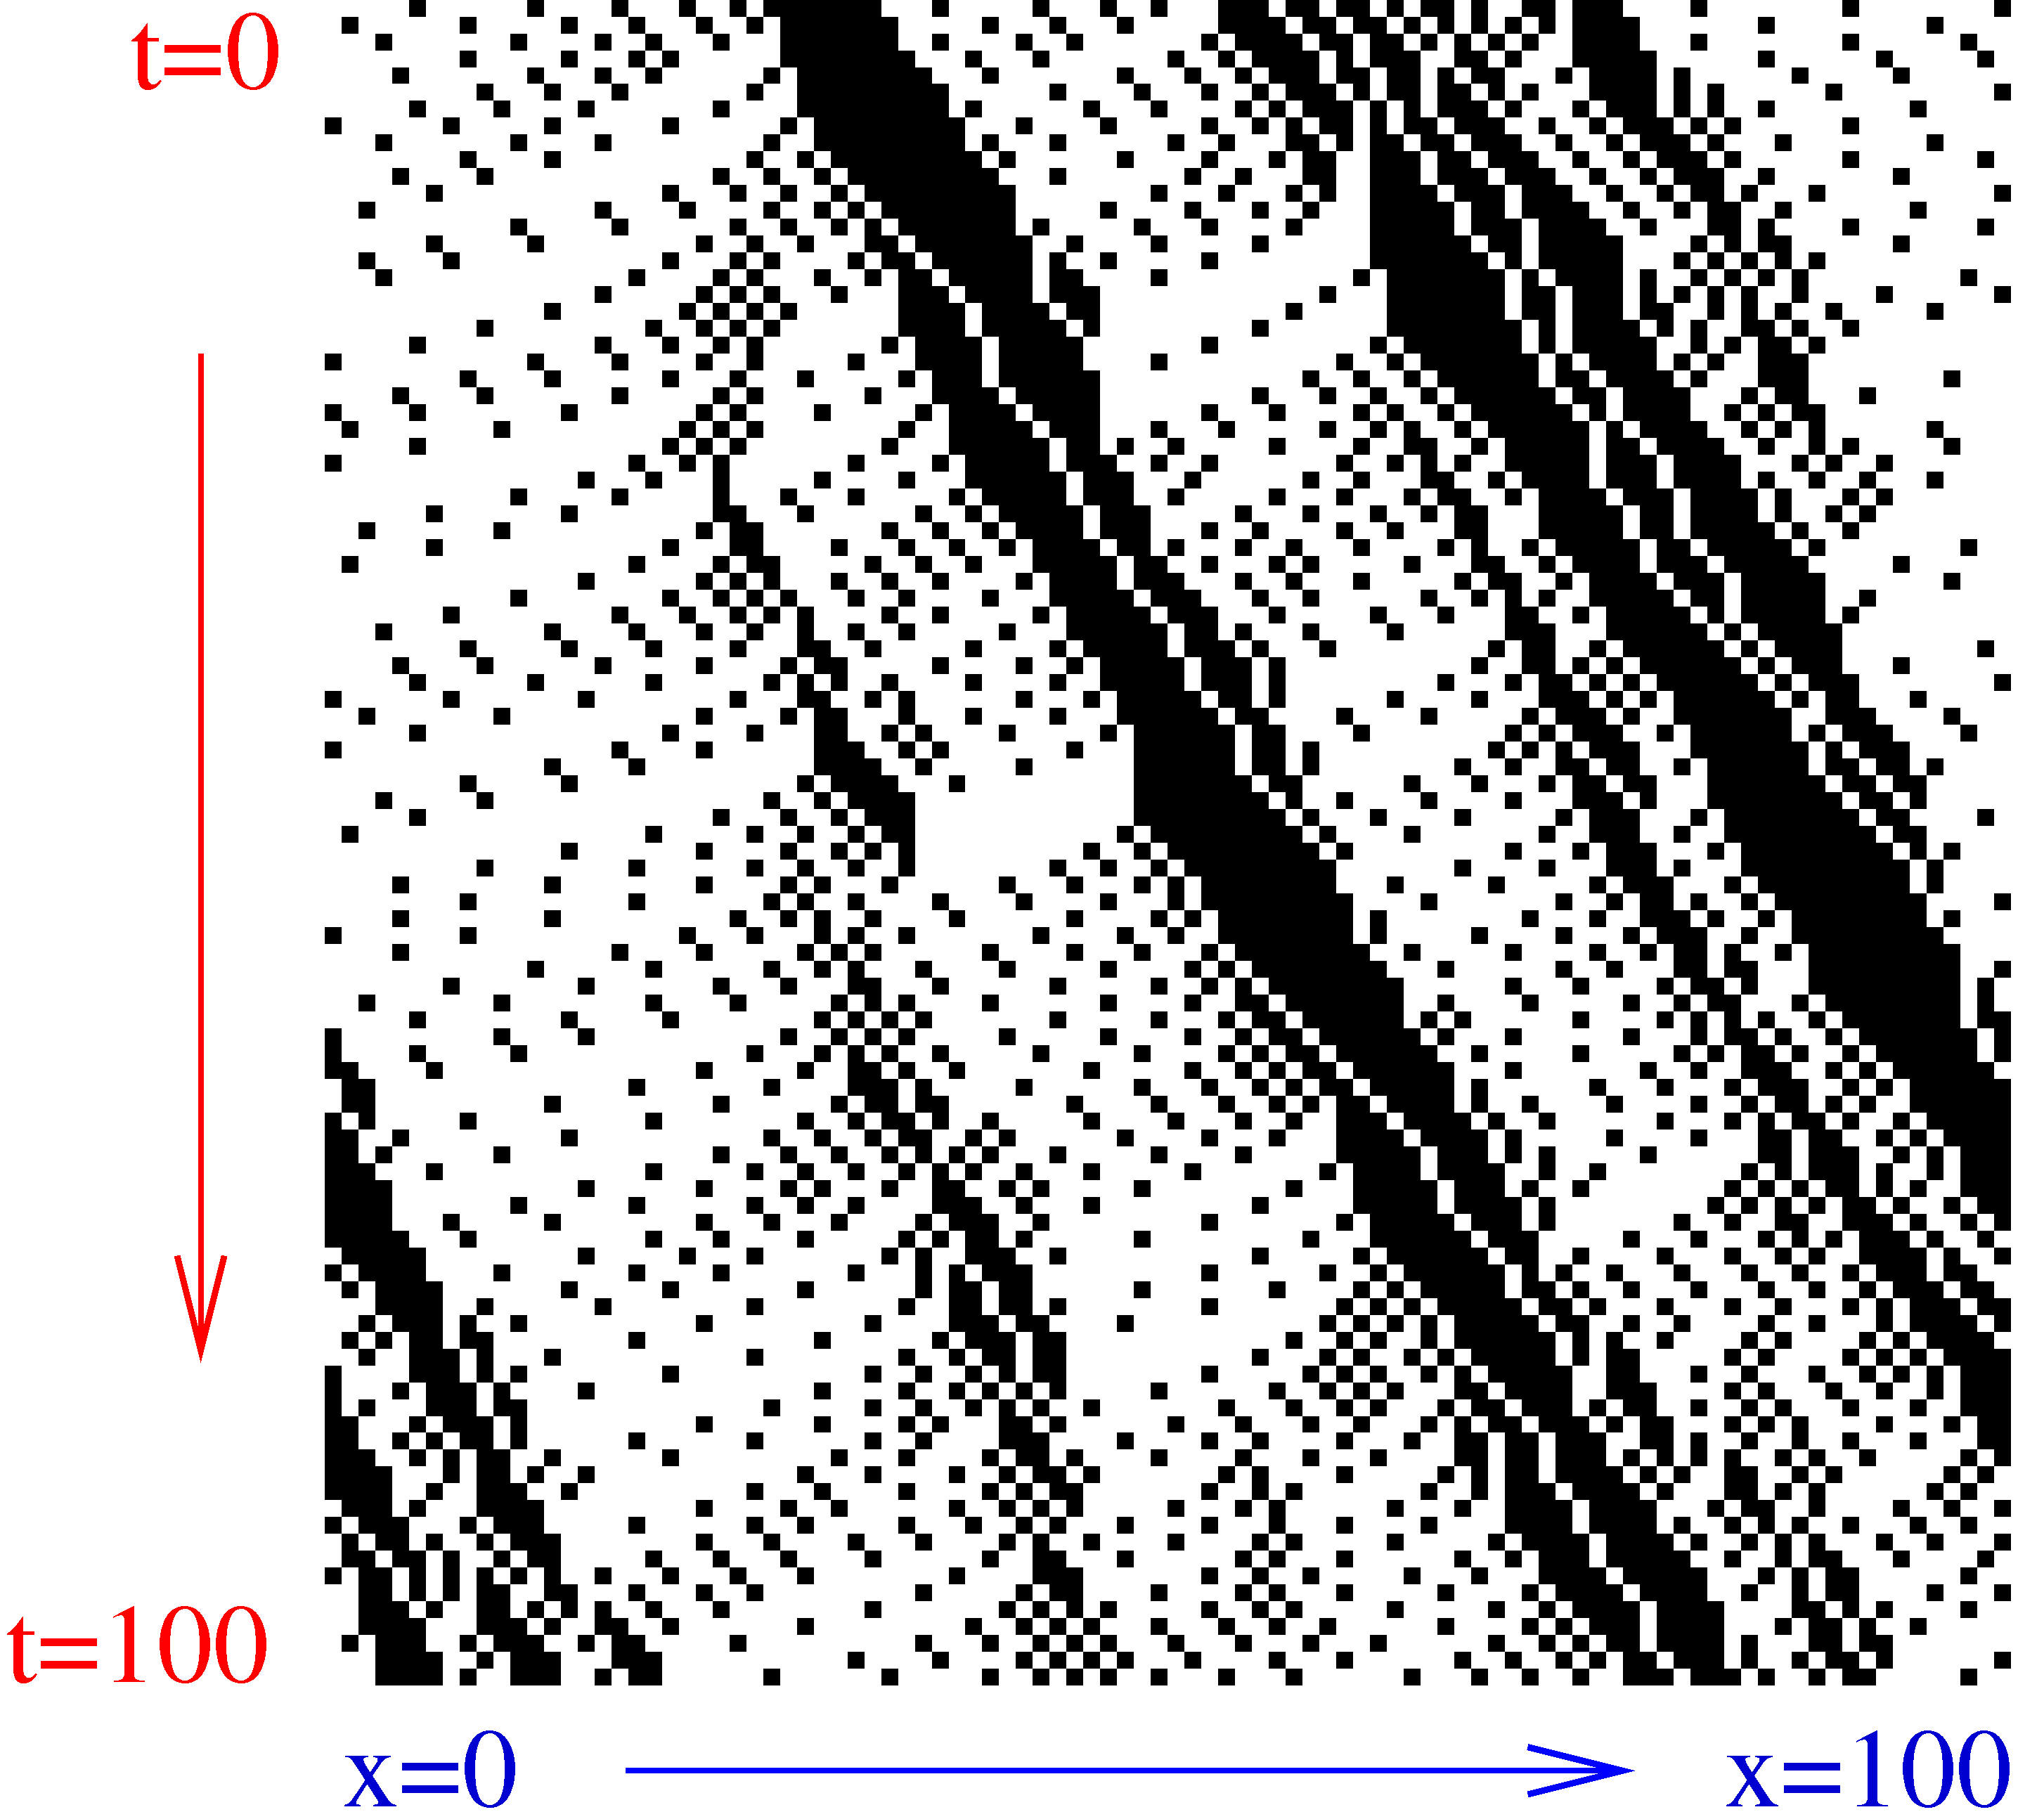
\includegraphics[width=.75\linewidth]{images/nagel-schreck}
	\caption{Representación de la evolución de un atasco en una autopista  de $100$ celdas de longitud usando el modelo Nagel-Scherckenberg. Con una densidad de ocupación $\rho = 0.35$ y una probabilidad de frenada de $p = 0.35$ se puede observar en la figura cómo se desplazan las olas del atasco a lo largo de los $100$ ciclos de la simulación. Feunte: Wikimedia}
	\label{fig:nagel-schreck}
\end{figure}

El modelo clásico de esta aproximación es el de Nagel-Scherckenberg (\cite{Nagel1992}), un modelo teórico creado para la simulación de tráfico en autopistas. La figura~\ref{fig:nagel-schreck} muestra la evolución del tráfico en una autopista a lo largo del tiempo de un autómata de este tipo. El resúmen de su funcionamiento es el siguiente:

\begin{itemize}
	\item La vía está divida en celdas de longitud $7,5m$ debido a que esta distancia es la media entre los parachoques traseros de dos coches consecutivos en un atasco.
	\item La celda puede tener dos estados, vacía o con un coche a una velocidad $v = \{0, \ldots, v_{max}\} \in \mathbb{N}$, esto es, discreta. La unidad de medida es $c/\Delta t$ siendo $c$ un número de celdas.
	\item $\Delta t$ queda establecido en $1s$, considerado el tiempo medio de reacción de un conductor ante una eventualidad. Esto hace, por ejemplo, que una velocidad de $6 c/\Delta t$ sea $45 m/s$ ($162 km/h$).
	\item En cada ciclo, se realizan cuatro acciones de manera simultánea: acelerar (nua unidad si no están a la máxmia velocidad), frenar (si se ven obligados en función de la velocidad y la distancia del siguiente vehículo), freno aleatorio (con una probabilidad de $p = 0.5$ la velocidad se reduce en una unidad hasta un mínimo de $v = 1 c/\Delta t$) y reposicionamiento (se avanzan tantas celdas como indica la velocidad.)
\end{itemize}

En general los modelos de la literatura suelen ser una variación de éste con ligeras modificaciones para estudiar aspectos concretos de modelos de tráfico, como la modificación del paso de \textit{aleatorización} (e.g. \cite{Barlovic1998}) o celdas más pequeñas (e.g. \cite{Krauss1997}) para comprobar la metaestabilidad del flujo de tráfico, o modelos y reglas para vías de dos carriles (e.g. \cite{Brilon1999} en la figura~\ref{fig:cellular-automata-based-sim} y~\cite{Nagel1998}).

\subsection{Microsimulación basada en sistemas multiagentes}

Los modelos basados en autómatas celulares, aunque interesantes, no son suficientemente realistas desde un punto de vista microscópico. Por poner un ejemplo, en una situación típica de un modelo Nagel-Scherckenberg, las posiciones de los vehículos se dan en últiplos de $7,5$ metros. Además, un vehículo realiza aleatoriamente aceleraciones y deceleraciones de $27 km/h$. Incluso en una situación favorable, cualquier vehículo puede realizar una aceleración de $0$ a $162km/h$ en sólo $6$ segundos. Por tanto, no ofrecen una visión fiable en caso de querer realizar estudios muy detallados del tráfico a nivel micro.

Una de las principales razones por las que usar un sistema multiagente como modelo en simulación es que cada uno de los individuos o "agentes" tienen su propia entidad dentro del sistema. Esto es, perciben tanto el entorno como el resto de agentes y actúan de acuerdo a lo percibido y a su comportamiento preestablecido. Basarse no sólo en las magnitudes físicas del resto de vehículos (e.g. distancia, aceleración, \ldots) sino también en un comportamiento de conducción ofrece un interesante campo de estudio a nivel cognitivo. El paradigma de los sistemas multiagentes se desarrolla en detalle en el capítulo \ref{ch:sota-agents-and-mas} y los comportamientos concretos de los agentes de interés para esta tesis en el capítulo~\ref{ch:sota-behavior-models}. Por tanto, este apartado únicamente hará una pequeña introducción a estudios existentes y aplicaciones de simuladores basados en este modelo.

\begin{figure}
	\centering
	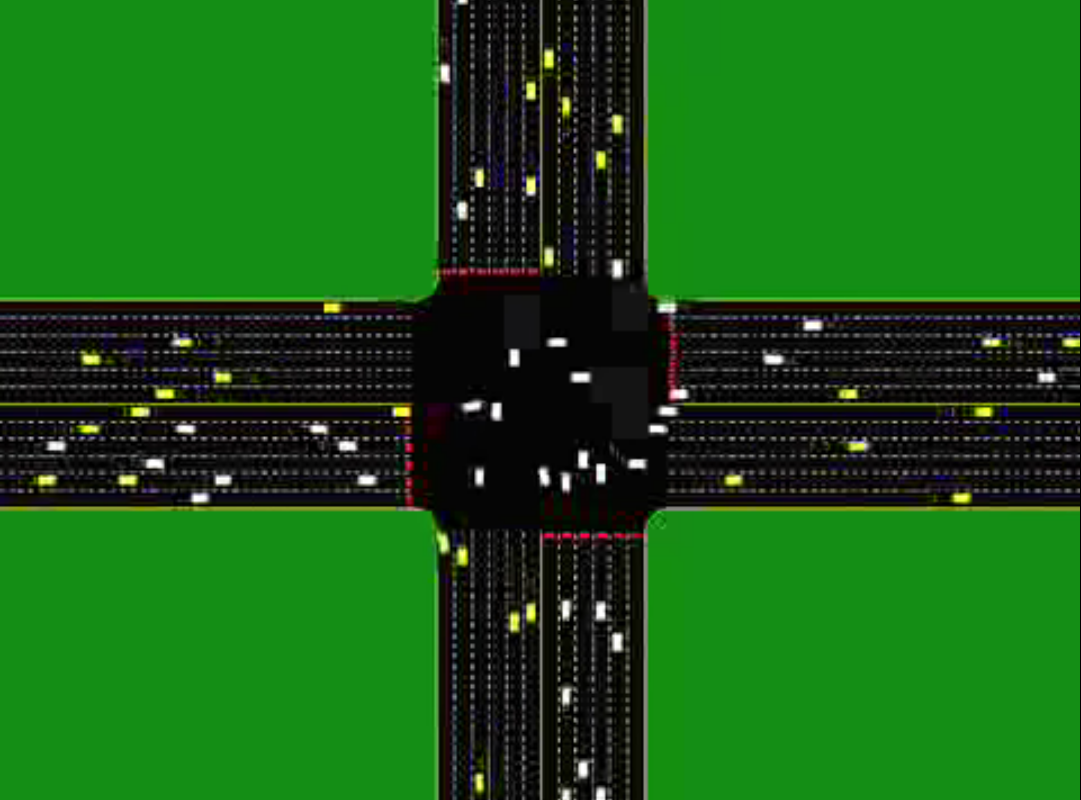
\includegraphics{images/autonomous-vehicles-at-intersections}
	\caption{Simulación de comportamiento en intersección basada en un modelo ultiagentes. Cada vehículo es un agente que representa, en este caso, el comportamiento de un coche autónomo. Fuente: Proyecto AIM (\url{http://www.cs.utexas.edu/~aim/}).}
	\label{fig:autonomous-vehicles-at-intersections}
\end{figure}

A diferencia de los autómatas celulares, los sistemas multiagentes pueden emplazarse en un entorno virtual que represente un espacio continuo y no discreto. Esto permite modelar con mayor fidelidad magnitudes físicas asociadas a cada agente (e.g. posición y velocidades actuales, dimensiones del vehículo, masa, velocidad máxima permitida, \ldots). Sin embargo, aun así no es una propiedad inherente de éstos. No existe ninguna limitación en cuanto a la representación del espacio y es perfectamente posible representar un modelo basado en autómatas celulares usando para ello un sistema multiagente.

Cada uno de los agentes es independiente del resto (y una consecuencia directa es que el comportamiento de acda individuo permite evaluar el comportamientos grupales complejos, como el que se describe en la figura~\ref{fig:autonomous-vehicles-at-intersections}). Esta independencia da la posibilidad de tener todos los agentes diferentes entre sí. Aunque de por sí la utilidad de este hecho no tiene por qué ser una ventaja, sí que lo es el poder experimentar con diferentes perfiles de conducción (e.g. un perfil agresivo en un flujo de tráfico dominado por conductores tranquilos). Esto es debido a que en un sistema multiagente cada agente es una parte del sistema y las decisiones de cómo se ha de comportar un agente se toman desde el propio agente. Desde el punto de vista de un autómata celular, el comportamiento existe en cada celda, dando control parcial o diretamente no dando control al estado de cada celda.

En general los estudios basados en este modelo suelen seguir el patrón $1$ DVU, $1$ agente\sidenote{Existe también una aproximación de modelar agentes como zonas de la vía y donde los vehículos, aunque poseen comportamiento, lo poseen gracias al agente que les guía de acuerdo a la zona en la que se encuentran. Esto tiene la ventaja de que el paso de información a vehículos dentro de la misma zona se realiza mucho más rápido en un entorno distribuido. Para más información, en \cite{Galis2000} se implementa un simulador siguiendo este concepto.}, dando así una enorme cantidad de posibilidades a experimentar. Por ejemplo en \cite{Das} se hace uso de sistemas difusos para decidir cómo comoprtarse en la vía mientras que en \cite{Ehlert2001} (\TODO{lo mismo cuentan los mismo que aquí: \cite{Ehlert2001-2}. Si es así, me tengo que zumbar uno de los dos) se hace uso de un patrón reactivo. Otros, como \cite{Dia2002} o \cite{Balmer} hacen uso de encuestas o censos para establecer las propiedades y calibrar los parámetros de diferentes tipos de agentes.

\begin{figure}
	\centering
	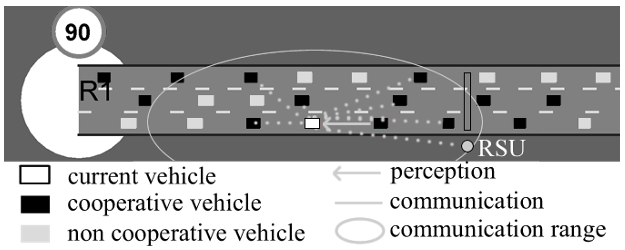
\includegraphics{images/cooperative-traffic-movsim}
	\caption{Captura de pantalla del simulador MovSim. Este simulador implementa un modelo multiagente donde los vehículos incorporan sistemas de comunicación vehicular. El estudio se centra en el uso de la comunicación entre vehículos para el acoplamiento dinámico de vehículos en sus respectivos carriles. Fuente: \cite{Gu2015}.}
	\label{fig:cooperative-traffic-movsim}
\end{figure}

Los estudios en materia de simuladores de tráfico con sistemas multiagente no se limitan a vehículos, sino que se usan también en áreas como el control de luces de tráfico o agentes para peatones entre otros. Un ejemplo es el estudio presentado en~\cite{Clymer2002} donde los agentes del sistema son las señales de tráfico luminosas y no los vehículos, y donde el objetivo es adaptar la señalización en una red de carreteras para minimizar al máximo el tiempo de espera por parte de los vehículos en las intersecciones gestionadas por las señales.

En los últimos años, otro concepto que está en auge es el de las comunicaciones extravehiculares (V2I) e intervehiculares (V2V). El modelo de sistemas multiagente permite la implementación rápida de diferentes políticas y protocolos de comunicación via sensores y actuadores para estudiar estos tipos de redes de comunicación (ver figura~\ref{fig:cooperative-traffic-movsim}). En~\cite{Shiose2001}\cite{Galis2000}, por ejemplo, se hace uso de un sistema multiagente para implementar diferentes formas de comunicación intervehicular con el objetivo de aliviar congestiones de tráfico (en el primer caso) y por el propio estudio de las comunicaciones en si (en el segundo caso). En el caso de redes extravehiculares, un buen ejemplo es~\cite{Dresner2004}, donde se representan como agentes tanto los vehículos como las intersecciones de la vía. Éstas gestionan un sistema de reservas que los vehículos que van a entrar en la intersección solicitan, gestionando  comunicando en todo momento mediante eventos los cambios en dicho sistema. El estudio concluye que una comunicación de este tipo es más eficiente que una intersección clásica basada en señales de tráfico luminosas.

\section{El vehículo como agente inteligente}

En nuestra tesis el trabajo se basa en la representación del comportamiento de un conductor. Para simplificar el problema asumiremos que los términos \enquote{conductor} y \enquote{vehículo} son equivalentes y que se refieren a la tupla \enquote{(vehículo, conductor)} (Hay un paper que lo denomina DVU como driver-vehicle-unit \cite{Dia2002})

No sé cómo ponerlo, pero esta información puede ser útil aquí. A lo mejor hay que separarlo, no sé. Yo lo pongo aquí porque me ha venido ahora.

\begin{itemize}
	\item \textbf{Percepción}. Característica intrínseca a todo ser vivo para la obtención de información del entorno. Pues para los agentes inteligentes, lo mismo. Puede ser en forma de sensores (e.g. sensor de velocidad, acelerómetro, sensor de distancia, lidar, cámaras, termómetros, gps, \ldots), conocimiento (e.g. controlador difuso, sistema experto, red neuronal, es decir, información procesada que ad valor añadido), datos GIS, comunicación con otros vehículos (e.g. V2V, V2E, \ldots). Un simulador nos ofrece estos sensores casi gratis, pero nuestro problema es que para la generación de modelos necesitamos previamente haber capturado información con dichos sensores y en físico ya es otra cosa.
	\item \textbf{Toma de decisiones}. Un agente racional en un sistema multiagente ha de ser capaz de razonar acerca del mundo, de su propio estado y del estado del resto de agentes.
	\item \textbf{Actuación}. La actuación es la consecuencia natural de las anteriores características. Dado un estado del mundo y un proceso cognitivo surgen acciones a realizar, tras las cuales se llega a un nuevo estado del entorno que provee de información actualizada para seguir actuando.
\end{itemize}

\section{Software de simulación}

Para la realización de al tesis es encesario contar con un paquete de simulación que permita modelar un sistema multiagente en el que poder ejecutar los modelos de comportamiento desarrollados.

Aunque en un principio se ha valorado el desarrollo de una solución propia, la oferta de simuladores en el mercado es muy amlpia, cada uno de ellos implementando nuo o varios modelos diferentes y bajo muy distintas licencias. Por ello se ha optado por la elección de un simulador ya existente.

Para elegir el mejor simulador que se adapte a nuestras necesidades se ha realizado un listado de características obligatorias para realizar una primera criba eliminando simuladores no aptos:

\begin{enumerate}
	\item \textbf{Tipo de simulador}. Al menos debe ofrecer un entorno de \textbf{microsimulación} de \textbf{espacio continuo} y \textbf{tiempo discreto}. Para nuestras necesidades es necesario un simulador que implemente microsimulación, ya que es el único tipo de granularidad que permite evaluar el comportamiento de un conductor independientemente del resto de la simulación. Además, debido a la forma en la que se recolectan los datos, es necesario que represente un espacio continuo y una dimensión de tiempo discreto con una resolucińo de al menos $1$ segundo.
	\item \textbf{Modelo de simulación}. Debe ofrecer un entorno basado en un \textbf{sistemas multiagente} donde cada vehículo se comporte como un agente individual.
	\item \textbf{Entorno de simulación}. Debe ofrecer un entorno de simulación de tráfico general, permitiendo la creación de escenarios. Quedan excluídos los simuladores de propósito específico o de casos particulares como simuladores de autopistas, congestiones o colisiones.
	\item \textbf{Extensibilidad}. El simulador debe permitir extender de alguna la ejecución de los modelos desarrollados en los agentes (DVUs). Aunque se puede considerar que si es simulador Open Software, es posible modificar su comportamiento para adcuarlo a los modelos desarrollados, es mejor que el propio software ofrezca los mecanismos necesarios para la integración sin necesidad de tocar los fuentes del sistema.
	\item \textbf{Sistema operativo}. Es imprescindible que el software se ejecute sobre sistemas operativos GNU/Linux por la configuración de los sistemas sobre los que se trabaja.
\end{enumerate}

Posteriormente se ha desarrollado un listado de características deseables. No son determinantes para descartar simuladores pero sí favorecen la elección de unos sobre otros.

\begin{enumerate}
	\item \textbf{Activo}. Es preferible que el sistema esté activamente desarrollado porque eso favorece la aparición de parches y mejoras sobre el software. En caso contrario, se trata de un proyecto con poca actividad por parte de sus autores.
	\item \textbf{Lenguaje de programación}. Es favorable la implementación de los modelos en código Python.
	\item \textbf{Licencia}.Es preferible una licencia de tipo Open Software (\TODO hay que ver si esto está bien dicho o no) ya que, en caso de error o falta de funcionalidad, es posible acceder a los fuentes para modificarlos.
	\item \textbf{Sistema operativo}. Es favorable que el sistema se ejecute en entornos tipo OS-X.
\end{enumerate}

\subsection{Entornos de simulación a estudiar}

El primer listado de características deja atrás la mayoría de simuladores (una gran cantidad de ellos son o bien de propósito específico, están desarrollados para sistemas operativos Windows o no permiten extender su modelo). Tras la selección, nos quedamos con dos simuladores:

\begin{table}
	\caption{Tabla comparativa cmoparando las característiacs deseables en los dos simuladores escogidos.}
	\label{tbl:simulators-comparison}
	\begin{tabular}{lllll}
		\toprule
		& Matsim & \acrshort{sumo} & \\
		\midrule
		Activo & \yep & \yep & \\
		\addlinespace
		Lenguaje de programación & Java & C/C++/Python & \\
		\addlinespace
		Licencia & & & & \\
		\quad Propietaria    & \yep & \yep \\
		\quad Open Software  & \yep & \yep \\
		\quad Compatible GPL & \yep & \yep \\
		\addlinespace
		Sistema operativo & & \\
		\quad GNU/Linux & \yep & \yep \\
		\quad OS X & \yep & \yep & \\
		\quad Windows & \yep & \yep \\
		\bottomrule
	\end{tabular}
\end{table}

\begin{enumerate}
	\item \textbf{MatSIM} (Multi-Agent Transport Simulation). Software de simulación multiagente desarrollado en la ETH Zürich. Url: \url{http://matsim.org}.
	\item \textbf{\ac{sumo}}. Entorno de simulación de granularidad micro y meso desarrollado por el instituto de sustemas de transoprte del DLR (Centro Aeroespacial Alemán). Url: \url{http://www.dlr.de}.
\end{enumerate}

Ambos entornos están igualados en las características presentadas, tal y como se puede observar en el cuadro~\ref{tbl:simulators-comparison}. Tras haber probado ambos simuladores hemos llegado a la conclusión de que \ac{sumo} y no matsim es el simulador que se usará en las simulaciones.

La razón es la facilidad con la que implementar los agentes. Mientras que MatSIM ofrece un API para desarrollar nuevas funcionalidades, no se ha encontrado forma para hacer lo mismo con los comportamientos de los vehículos. Por tanto sería necesario modificar los fuentes del simulador. SUMO por otro lado permite la programación de los agentes a través la librería externa TraCI en Python.

\subsection{Entorno seleccionado: \acrshort{sumo}}

En definitiva, el simulador que más se adapta a nuestras necesidades y el que se usará como simulador base en el desarrollo de esta tesis será \gls{sumo}\sidenote{Sus principales publicaciones son~\cite{krajzewicz2002sumo}, \cite{behrisch2011sumo} y \cite{krajzewicz2012recent}.}. \gls{sumo} es un entorno de microsimulación de código abierto\sidenote{Licenciado bajo la \gls{gpl}, concretamente la versión $3.0$.} que implementa un modelo discreto en el tiempo y continuo en el espacio.

Además de simulación clásica, \gls{sumo} provee de una interfaz gráfica (se puede ver una captura de la vista gráfica en la figura~\ref{fig:sumo-simulator}) donde se puede ver el comportamiento de cada vehículo durante la simulación. Es interesante para obtener de un vistazo información acerca del funcionamiento del modelo en concreto a controlar. Otras de las características que el simulador ofrece son las siguientes:

\begin{figure}
	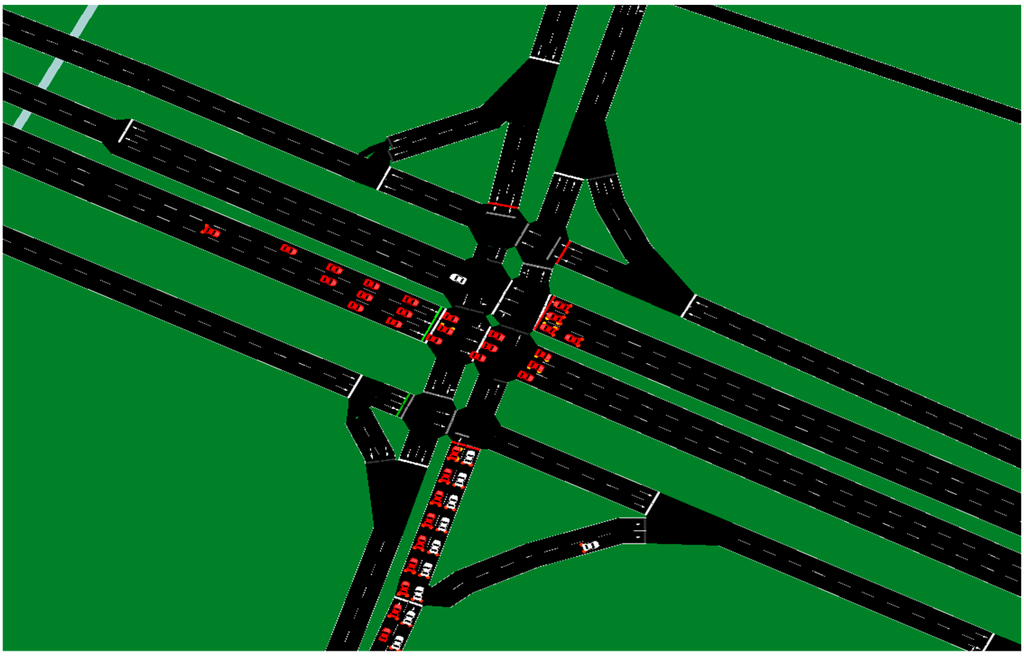
\includegraphics{sumo-simulator}
	\caption{Ejemplo de pantalla del simulador \gls{sumo}. Además de entorno de simulación propiamente dicho, \gls{sumo} provee de una interfaz gráfica que permite una visualización general, de zonas y de elementos en concreto a la vez que permite la variación de configuración de la simulación durante el desarrollo de la misma.}
	\label{fig:sumo-simulator}
\end{figure}

\begin{itemize}
	\item Multimodalidad permitiendo modelar no sólo tráfico de vehículos sino de peatones, bicicletas, trenes e incluso de barcos.
	\item Vehículos de diferentes tipologías, Simulación con y sin colisiones de vehículos.
	\item Diferentes tipos de vehículos y de carreteras, cada una con diferentes carriles y éstas con diferentes subdivisiones de subcarriles (diseño conceptual para permitir las simulaciones )
\end{itemize}

Al estar licenciado bajo la licencia \gls{gpl}, su distribución implica a su vez la distribución de su código fuente. Esto permite la modificación de su comportamiento y el desarrollo de nuevos modelos integrados dentro del simulador. Sin embargo nosotros no haremos uso de esta característica, sino que usaremos \gls{sumo} como aplicación servidor y el módulo \gls{traci} como aplicación cliente desde donde gestionar todos los aspectos de cada simulación.

\subsection{La interfaz \glsentrylong{traci}}

\gls{traci} (\cite{Wegener2008}) es tanto el nombre del protocolo de comunicación expuesto por \gls{sumo} en su versión servidor como el nombre de la librería escrita en Python para interactuar con el mismo.

Como protocolo, la interacción a través de cliente/servidor comienza especificando a \gls{sumo} que se desea trabajar de este modo. En ese momento, \gls{sumo} se inicializa en modo servidor dejando abierto un puerto TCP para la conexión del cliente.

Una vez el servidor se encuentra en ese estado, el cliente se conecta enviando una señal de conexión indicando que él se encargará de controlar la simulación. Desde ese momento y hasta que el cliente no envíe una señal de desconexión, el cliente podrá enviar y recibir todos los mensajes que desee para capturar información y modificar los detalles de la simulación, incluido el mensaje \textit{step}, que es el encargado de avanzar un paso en la simulación. . Podemos ver un ejemplo en la figura~\ref{fig:traci-messages} dnode se dan tres ejemplos de mensajes enviados a \gls{sumo} a través de \gls{traci}.

\begin{figure}
	\centering
	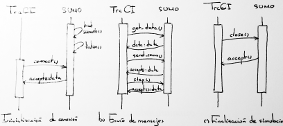
\includegraphics{images/traci-messages}
	\caption{\gls{sumo} ofrece la posibilidad de interactuar con la simulación desde cualquier aplicación a través del uso del protocolo \gls{traci}. En la figura podemos ejemplos de comunicación como (a) la incialización, (b) una petición de información acompañada de una modificación de comportamientoseguida de una solicitud de avanzar la simulación un paso o (c) una finalización de simulación.}
	\label{fig:traci-messages}
\end{figure}

Como implementación, \gls{traci} es una librería desarrollada en Python XX, aunque no es la única. Si bien es cierto que es posible trabajar directamente con el protocolo de comunicación a través de sockets, una librería abstrae todos los detalles dando una interfaz de trabajo más clara y sencilla. Por ello, aunque no se usarán en la tesis, existen otras dos implementaciones que merece la pena mencionar:

\begin{itemize}
	\item \textbf{TraCI4J}. El homólogo de la librería de abstracción de Python pero para el lenguaje Java. Está desarrollada por un tercero. Url: \url{https://github.com/egueli/TraCI4J}.
	\item \textbf{TrasS}. Una plataforma ofrecida como SaaS que proporciona una interfaz de servicios web bajo protocolo SOAP para abstraer el protocolo en mensajes HTTP (figura~\ref{fig:traas}). Url: \url{http://traas.sourceforge.net/cms/}.
\end{itemize}

\begin{figure}
	\centering
	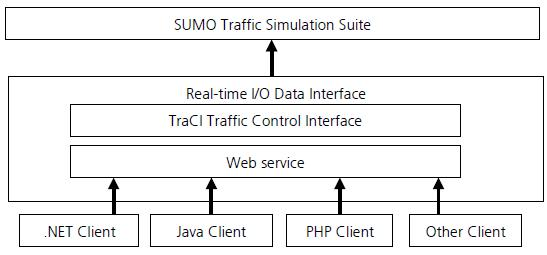
\includegraphics{images/traas}
	\caption{Concepto arquitectural de la plataforma TraaS. La plataforma se conecta como cliente a \gls{sumo} y ofrece un API basado en SOAP de mensajes que traduce en mensajes del protocolo \gls{traci}, lo que independiza completamente la elección de lenguaje de programación a la vez que abstrae los detalles del protocolo de comunicación.}
	\label{fig:traas}
\end{figure}
